\section{System Overview} \label{sec-overview}

Inspired by the problem caused by outliers, we name our system NO Outliers ($NO^2$) which implies our
wishes as well as indicates $NO^2$'s mission. It is learned that there is only one system which has a
similar name with $NO^2$ in the world.It is named N2O system, primarily concerning with
introducing fuel and nitrous into the engine's cylinders and combining which for more
efficient combustion. N2O system is typically used for providing an instantaneously speedup for auto.
Whereas, our $NO^2$ system can continuously speed up parallel processing for massive
compute-intensive tasks in clusters and clouds.

$NO^2$ contains two main components which are the instrumenter and tasks scheduling policy
generater. The instrumenter's perfect partner the instrument points selector
collects the statistics of function hits in a variety of executions and selects some
function entries for an appropriate instrumentation granularity. The instrumenter
can finish the instrument task of tracing all function entries by itself, additional overhead such
as some percentage of execution time is unavoidable. This is unacceptable in
production system. With the instrument points selector's cooperation, overhead can be
reduced to a low level, or even can be negligible. Details will be shown in the evaluation section. The
tasks scheduling policy generater is supported by the outliers clustering. With the
outliers information, an optimized tasks scheduling policy can be generated for the job
running on cluster. As shown in Fig.\ref{figure:no2arch}, users submit jobs with a job description which
configured for using instrumented binary code. The running instumented processes provide traces for
clustering outliers.

\begin{figure}
\centering
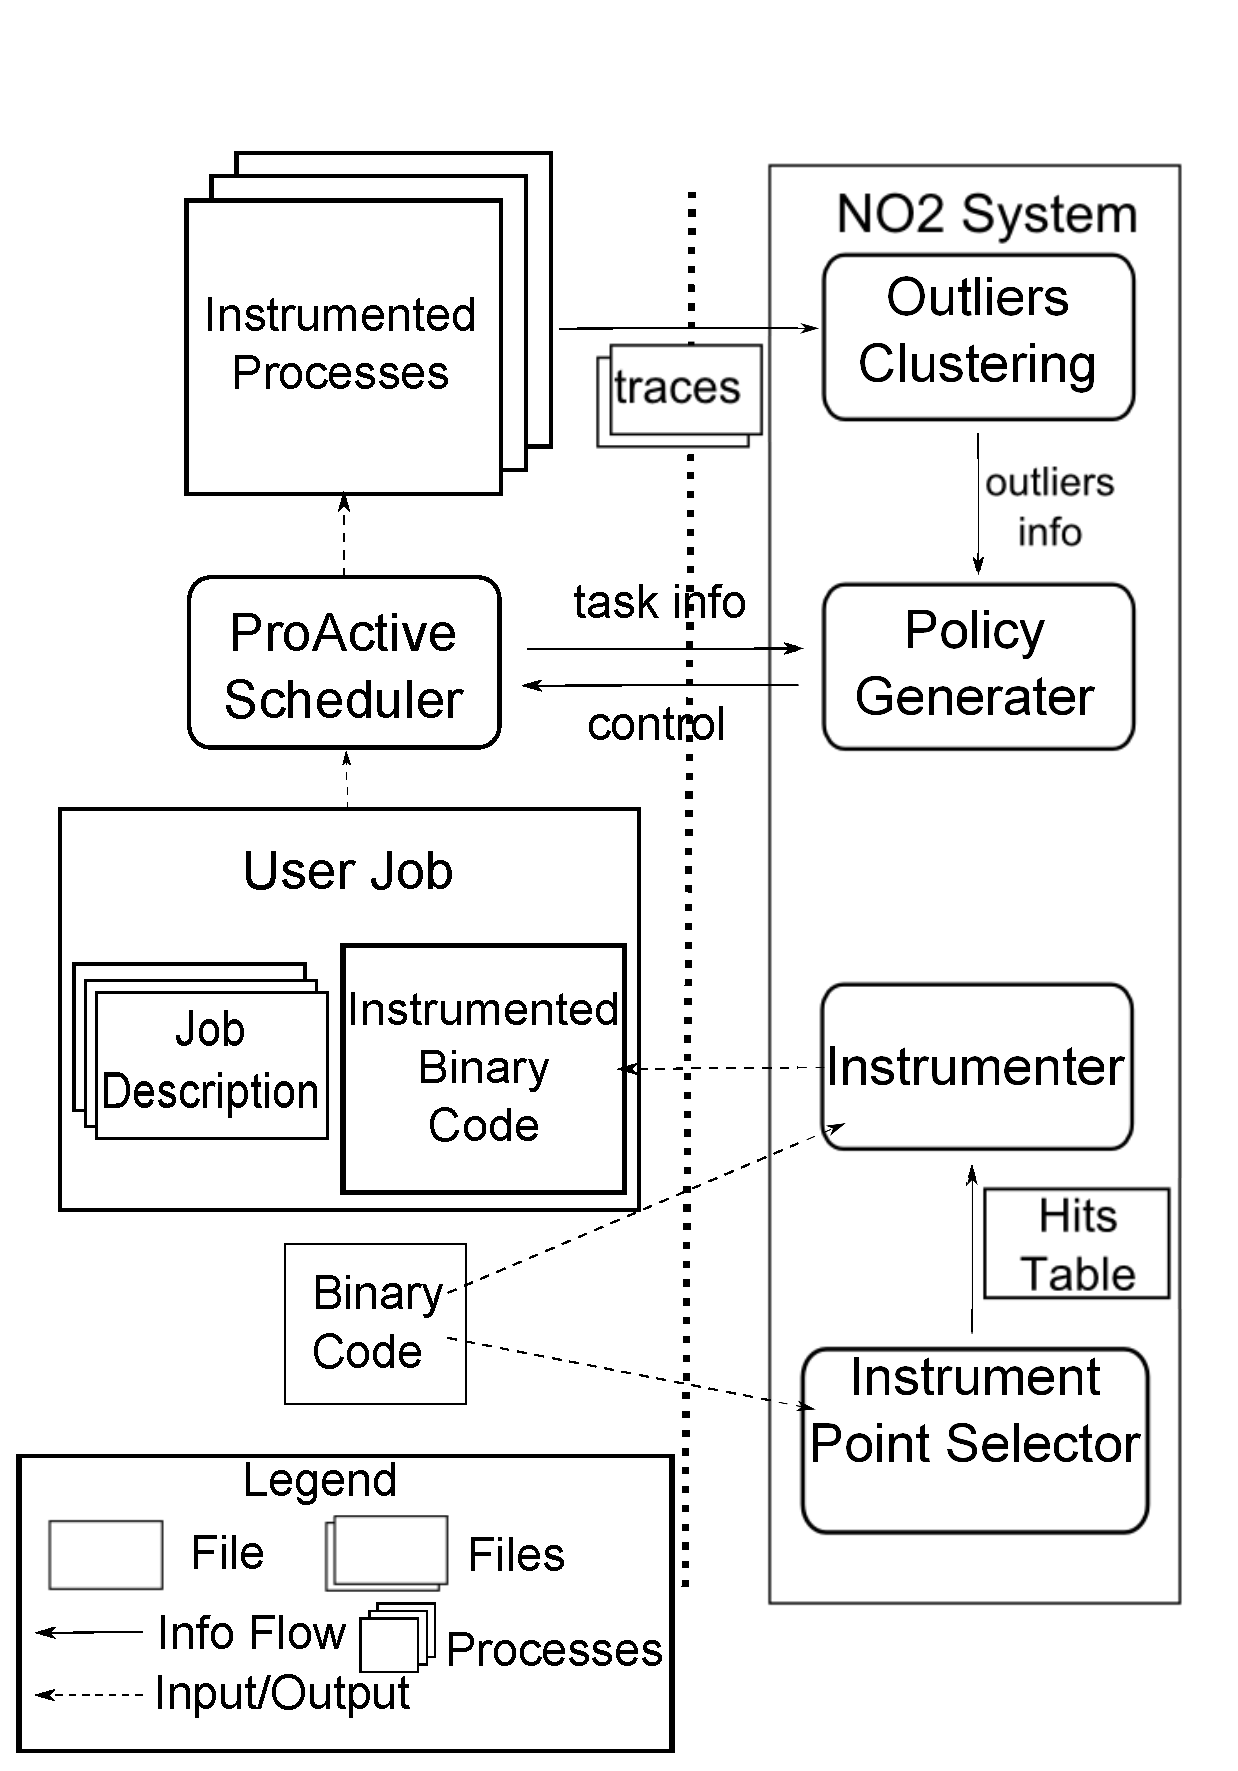
\includegraphics[width=0.9\columnwidth]{figures/NO2_arch.eps}
\caption{$NO^2$ architecture}
\label{figure:no2arch}
\end{figure}

We carefully designed $NO^2$ to assure its independence with the job scheduler that
facilitates users' adaptation to different job schedulers. As Fig.
\ref{figure:no2arch} shows, the only coupling between $NO^2$ and
ProActive Scheduler is interfaces for obtaining task status information of a job and
requesting to kill or start a task. These abilities can be easily satisfied by any job
scheduler's control interface, such as control script provided by ProActive Scheduler or
command line tools provided by Condor.

The instrumentation has two phases: function hits statistics and instrument with selected
functions by the instrument points selector. For function hit statistics, another
instrumentation is needed. As the statistics are offline, this instrumentation covers all
functions in the binary code without considering instrumentation overhead. The
modified binary code is executed with some input cases in production runs and
the statistic results are saved in a file. With the statistics, the instrumentation for progress
trace can be performed with the binary code in an appropriate granularity.

The speculation algorithm of tasks scheduling for a job is straightforward with a few of
heuristics improvement driven by several rules of thumb. These empirical rules are
reasonable and have been verified in practice. The first rule is to assign a higher speculation
priority to a worse outlier. As speculation is costly, this rule is obviously advisable. Making
sure that the split task and merge task do not execute on irregular nodes is another
important rule because we should not expose an outlier with a single task. On the
other hand, the split and merge phases are always the critical stage of a job. The last
one is to speculate as soon as possible without irregular nodes. The goal of speculation
is to complete the job early. Earlier and faster speculation means better opportunity. The
pseudo code of speculation algorithm is shown in Fig. \ref{fig-spec-algo}.

\begin{figure}
\rule[-.2pt]{0.9\columnwidth}{0.9pt}
\textbf{Algorithm:TasksSpeculation}
\rule[-.2pt]{0.9\columnwidth}{0.5pt}

\begin{algorithmic}[1]
\Require{instance of the $job$ and sleep $interval$}
\Ensure{the job's state $job.state$}

\While{$job.state\not=FinishedOrFaulty$}
    \State $tasks\gets job.tasks$
    \State $clusters\gets kmeans(tasks.traces, 2)$
    \If{$variance(clusters) > threshold$}
        \State $outliers\gets min(clusters)$
        \State $sort(outliers, comparePriority)$
        \For{$outlier \in outliers$}
            \State $s\gets submit(outlier.taskid)$
            \State $speculations\gets [speculations, s]$
        \EndFor
    \EndIf
    \State $sleep(interval)$
    \State $job.update()$
    \For{$s \in speculations$}
        \If{$s.state = Finished$}
            \State $kill(s.outlier.taskid)$
        \ElsIf{$s.outlier.state = Finished$}
            \State $kill(s.taskid)$
        \EndIf
    \EndFor
\EndWhile\label{specendwhile}
\end{algorithmic}
\rule[-.2pt]{0.9\columnwidth}{0.8pt}
\caption{Task speculation algorithm}\label{fig-spec-algo}
\end{figure}

In the next two sections, we will mainly illustrate the design of instrumentation based on
function hits statistics and outliers clustering, which are the two key points in $NO^2$. 